\documentclass[12pt,a4paper]{article}

\setcounter{secnumdepth}{3}
% USEPACKAGE LISTA
\usepackage[utf8]{inputenc}
\usepackage{amsmath}
\usepackage{mathtools}
\usepackage{marvosym} 
\usepackage{wrapfig}
\usepackage{hyperref}
\usepackage{float}
\usepackage{multicol}
\hypersetup{colorlinks,citecolor=black,filecolor=black,linkcolor=black,urlcolor=black}
\usepackage{pdfpages}
\usepackage{amsfonts}
\usepackage{amssymb}
\usepackage{hyperref}
\usepackage{fancyhdr}
\usepackage{graphicx}
\usepackage[export]{adjustbox}
\usepackage{t1enc}
\usepackage[english]{babel}
\usepackage{bm}
\usepackage{multirow}

\usepackage{booktabs}

\usepackage{pgfplots}
\pgfplotsset{height = 10cm, width=15cm,compat=1.9}

% \usepackage[usenames,dvipsnames]{xcolor}
\usepackage[left=2cm,right=2cm,top=2cm,bottom=2cm]{geometry}

\setlength{\parindent}{0pt} % bekezdés behúzása
\setlength{\parskip}{0em}   % bekezdések közti távolság
\pagestyle{fancy}
\fancyhf{}


% --> disable section num
% \setcounter{secnumdepth}{0}



\title{Continuum Mechanics\\(BMEGEMMNWCM)\\II. Homework}
\author{Szász Zsolt\\KRCH5Q}
\date{November 26, 2024}

\lhead{Szász Zsolt\\KRCH5Q}
\chead{}
\rhead{Continuum Mechanics\\II. Homework}
\cfoot{\thepage. page}

% ITT KEZDŐDIK A DOKUMENTUM



\begin{document}




\maketitle{}
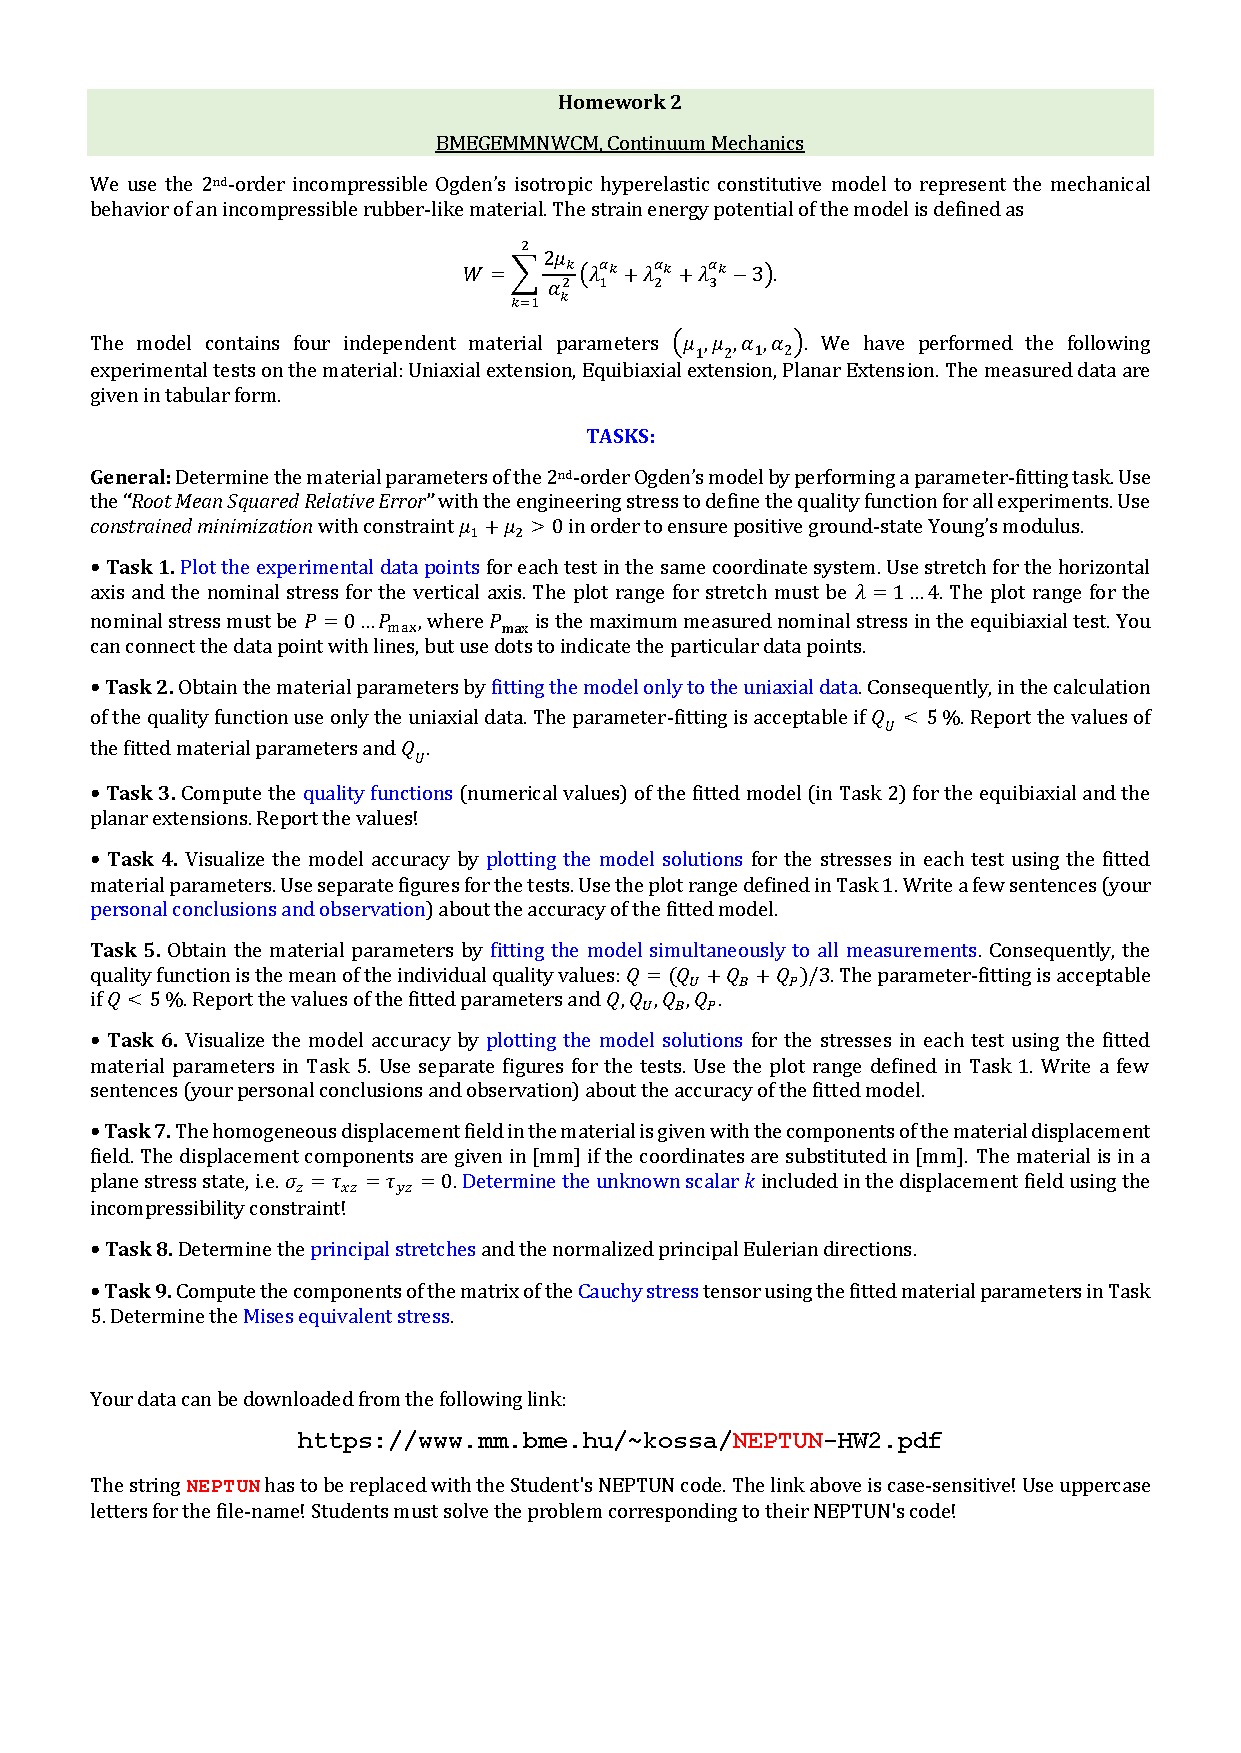
\includepdf[pages=-]{contmech_hw2.pdf}
\newpage
\tableofcontents

\newpage

\section*{Data}

Experimental data:\\

\begin{tabular}{rrrr}
    \toprule
    Eng. Strain  & Eng. Stress  (Uniaxial) & Eng. Stress  (Equibiaxial) & Eng. Stress  (Planar) \\
    \% & MPa & MPa & MPa \\
    \midrule
    0 & 0 & 0 & 0 \\
    30 & 6 & 10 & 7 \\
    60 & 8 & 17 & 10 \\
    90 & 9 & 22 & 12 \\
    120 & 11 & 28 & 14 \\
    150 & 12 & 37 & 16 \\
    180 & 14 & 44 & 17 \\
    210 & 15 & 52 & 19 \\
    240 & 16 & 60 & 21 \\
    270 & 17 & 70 & 23 \\
    300 & 19 & 82 & 24 \\
    \bottomrule
\end{tabular}
\\\\
Deformation:
$$
\boldsymbol{U} = 
\begin{bmatrix}
    5-3kX\\
    1+0.3X+0.5Y\\
    3\\
\end{bmatrix}
$$

\section{Task: Plotting experimental data}

Using the provided data, we can plot the experiments:

\begin{figure}[h]
    \centering
    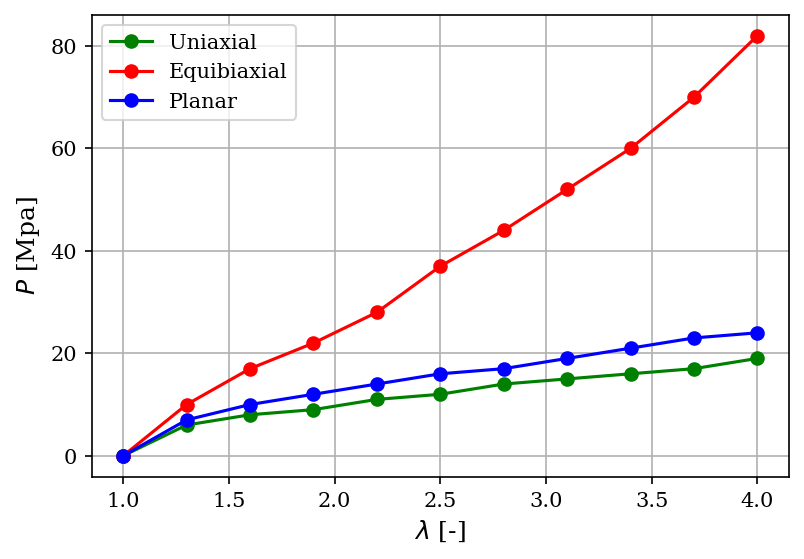
\includegraphics[scale=1]{figures/experiments.png}
    \caption{Experimental data}
\end{figure}


\section{Task: Fitting model only to the unaxial data}

At the lecture, we saw the solution of the general Ogden's model for the uniaxial tension, which in our 2nd order case looks like

$$
P^U_{OG} = \sum_{k=1}^2 \frac{2\mu_k}{\alpha_k}(\lambda^{\alpha_k - 1} - \lambda^{-\frac{\alpha_k}{2} - 1}).
$$

Based on the instruction we can define a quality function calculated from the given $n=11$ measured point, which looks like

$$
Q_U = \sqrt{\frac{1}{n}\sum_{i=1}^{n} \left(\frac{P^U_i-P^U_{OG}(\lambda_i)}{P^U_i}\right)^2}.
$$

Choosing this quality function as the objective function of an optimization algorithm, we can fit the model parameters to the provided data points. I will use the \texttt{scipy.optimize.minimize} function, with BFGS (Broyden-Fletcher-Goldfarb-Shanno) method. I will also apply the given $\mu_1 + \mu_2 > 0$ constraint. The optimialization results the following parameters:


\begin{table}[h]
    \caption{Parameters of model fitted only on uniaxial data}
    \centering
    \begin{tabular}{|c|c|c|c|}
    \hline
    $\mu_1$ [MPa]& $\mu_2$ [MPa]& $\alpha_1$ [-]& $\alpha_2$ [-]\\ \hline
    $10.71992575$   & $0.04956515$   & $-3.2772214$ & $4.57758998$   \\ \hline
    \end{tabular}
\end{table}

The quality functions value is

$$
Q_U = 3.2700839\;\% < 5\;\%
$$

\section{Task: Equibiaxial and planar quality functions}

The model response for the equibiaxial and planar loading was also shown at the lecture as

$$
P_{OG}^E = 
\sum_{k=1}^2 \frac{2\mu_k}{\alpha_k}(\lambda^{\alpha_k - 1} - \lambda^{-2\alpha_k - 1})
\quad\&\quad
P_{OG}^P = 
\sum_{k=1}^2 \frac{2\mu_k}{\alpha_k}(\lambda^{\alpha_k - 1} - \lambda^{-\alpha_k - 1}).
$$

With them we can define the quality functions regarding to equibiaxial and planar experiments too, like previously

$$
Q_E = \sqrt{\frac{1}{n}\sum_{i=1}^{n} \left(\frac{P^E_i-P^E_{OG}(\lambda_i)}{P^E_i}\right)^2}
\quad\&\quad
Q_P = \sqrt{\frac{1}{n}\sum_{i=1}^{n} \left(\frac{P^P_i-P^P_{OG}(\lambda_i)}{P^P_i}\right)^2}.
$$

Which can be evaluated with the model fitted to the uniaxial data

$$
Q_E = 7703.9478\;\%,
$$
$$
Q_P = 306.5815\;\%.
$$

We can observe the overfitting of the model to the uniaxial data points.

\newpage

\section{Task: Plotting solutions}

\begin{figure}[h]
    \centering
    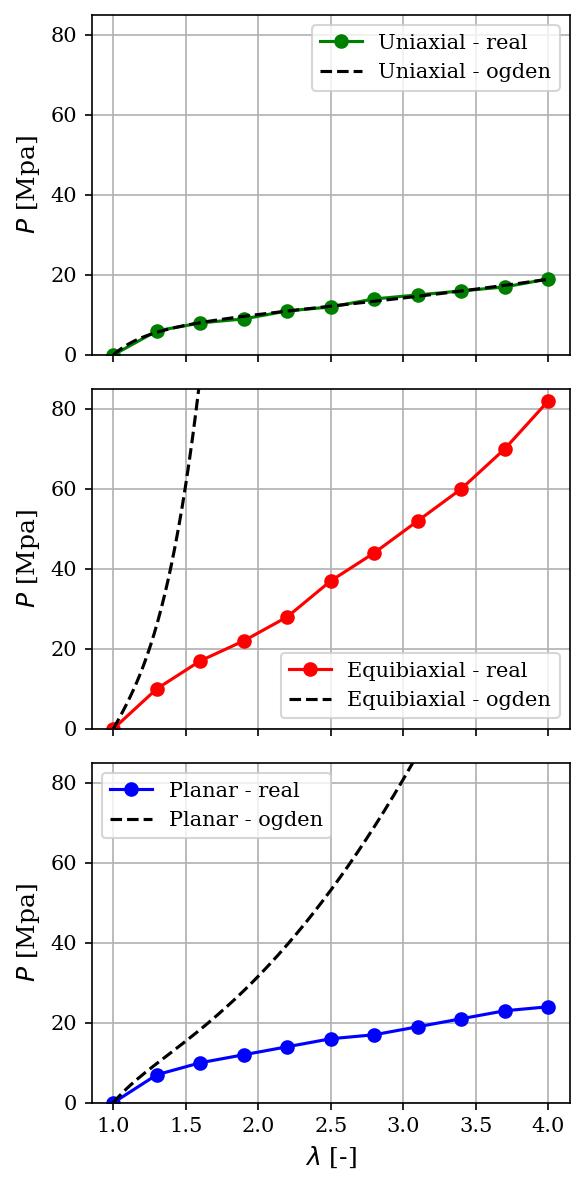
\includegraphics[scale=0.8]{figures/uniaxial_fit.png}
    \caption{Uniaxially overfitted model's response for uniaxial, equibiaxial and planar loads}
\end{figure}

We can observe how the model overfits to the uniaxial measurement data. The reason is that, we didn't take into account the error of the equibiaxial and planar quality functions during the optimization procedure.

\section{Task: Simultaneous fitting to all measurements}

To take into account the equibiaxial and planar measurements too, we will use the suggested 

$$
Q = \frac{Q_U + Q_B + Q_P}{3}
$$

objective function during the optimization. The procedure itself is tha same as the one used in the 2nd task. The resulting parametrs are

\begin{table}[H]
    \caption{Parameters of model fitted simultaneously to all measurements}
    \centering
    \begin{tabular}{|c|c|c|c|}
    \hline
    $\mu_1$ [MPa]& $\mu_2$ [MPa]& $\alpha_1$ [-]& $\alpha_2$ [-]\\ \hline
    $3.18596983$   & $4.62213918$   & $-1.48228961$ & $1.77455216$   \\ \hline
    \end{tabular}
\end{table}

The values of the objective and separate three quality functions looks like

$$
\begin{array}{llll}
    Q = 4.204376\;\% < 5\;\%&&& Q_U = 6.414038\;\% \\
    Q_E = 2.196516\;\% &&& Q_P = 4.002574\;\%
\end{array}
$$

\section{Task: Plotting solutions}

\begin{figure}[h]
    \centering
    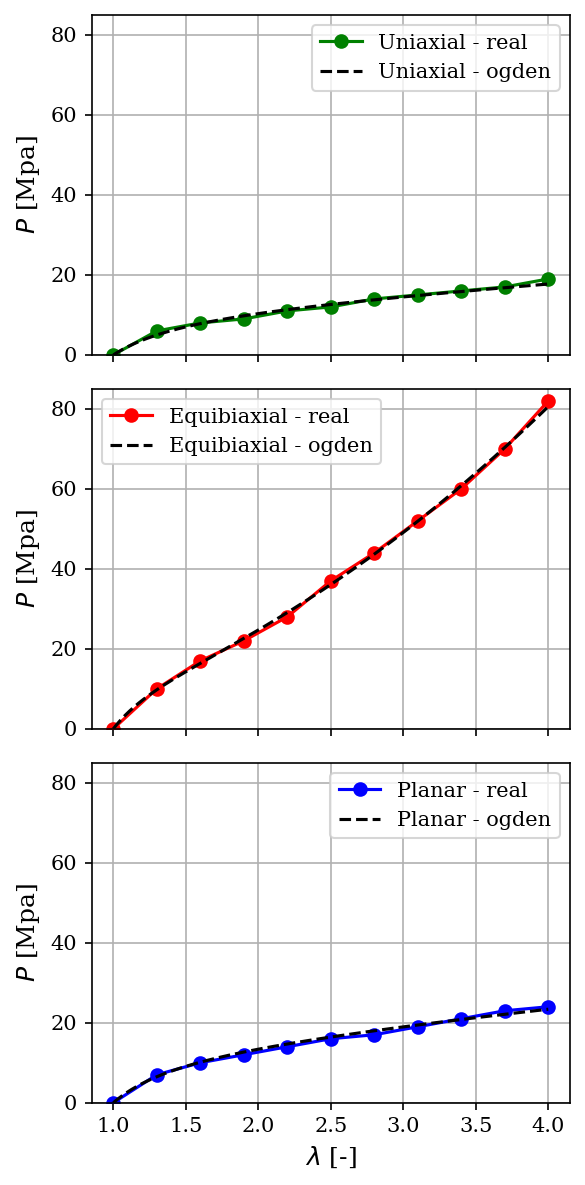
\includegraphics[scale=0.8]{figures/simultan_fit.png}
    \caption{Simultaneously fitted model's response for uniaxial, equibiaxial and planar loads}
\end{figure}

We can see that taking into account all of the measurement series in the objective, provide us a model which fit into all of the measuremet datas.

\newpage

\section{Task: Determination of k}

The displacement field is given in the with the components of the material displacement
field, like

$$
\boldsymbol{U} = 
\begin{bmatrix}
    5 - 3kX_1\\
    1 + 0.3X_1 + 0.5X_2 \\
    3
\end{bmatrix}.
$$

From here we can determine the displacement gradient as

$$
\boldsymbol{K} = \frac{\text{d}\boldsymbol{U}}{\text{d}\boldsymbol{X}} = 
\begin{bmatrix}
    -3k & 0 & 0 \\
    0.3 & 0.5 & 0 \\
    0 & 0 & 0 \\
\end{bmatrix}.
$$

The deformation gradient can be calculated as

$$
\boldsymbol{F} = \boldsymbol{K} + \boldsymbol{I} = 
\begin{bmatrix}
    1-3k & 0 & 0 \\
    0.3 & 1.5 & 0 \\
    0 & 0 & 1 \\
\end{bmatrix}.
$$

The volume change can be calculated as the determinant of the deformation gradient

$$
J = \text{det}\boldsymbol{F} = (1-3k)\cdot 1.5
$$.

If there is incompressible case, the volume change should be equal with 1, therefore:

$$
(1-3k)\cdot 1.5 = 1,
$$
$$
k = \frac{1}{9}.
$$

\section{Task: Principal streches}

We know that by the deformation gradient we can determine the left Cauchy-Green strain tensor as

$$
\boldsymbol{b} = \boldsymbol{F}\boldsymbol{F}^T = 
\left[\begin{matrix}0.444 & 0.2 & 0\\0.2 & 2.34 & 0\\0 & 0 & 1.0\end{matrix}\right].
$$

The eigendecomposition of the Cauchy-Green tensor looks like

$$
\boldsymbol{b} = \sum_{i=1}^3 \mu_i \cdot \boldsymbol{n_i} \otimes \boldsymbol{n_i} =  \sum_{i=1}^3 \lambda_i^2 \cdot \boldsymbol{n_i} \otimes \boldsymbol{n_i},
$$

where $\lambda_i$ are the principal streches and $\boldsymbol{n_i}$ are the principal Eulerian directions. They numerically looks like

$$
\begin{array}{ll}
    \lambda_1 = 0.65082 & \boldsymbol{n_1} = \left[\begin{matrix}-0.994599 & -0.103797 & 0\end{matrix}\right]^T \\
    \lambda_2 = 1.53651 & \boldsymbol{n_2} = \left[\begin{matrix}0.103797 & -0.994599 & 0\end{matrix}\right]^T\\
    \lambda_3 = 1 & \boldsymbol{n_3} = \left[\begin{matrix}0 & 0 & 1\end{matrix}\right]^T\\
\end{array}.
$$

\newpage

\section{Task: Cauchy stress tensor and Mises Equivalent stress}

When we're talking about plane stress problems, the Cauchy stress tensors reduces to

$$
\boldsymbol{\sigma} = 
\begin{bmatrix}
    \sigma_x & \tau_{xy} & 0\\
    \tau_{xy} & \sigma_y& 0\\
    0 & 0& 0\\
\end{bmatrix}
$$

First we should mention the decomposition of the stress tensor into deviatoric and spherical part, which looks like

$$
\boldsymbol{\sigma} = \boldsymbol{s} + \boldsymbol{p}
$$

because, we know that in hyperelasticity the deformation only determine the deviatoric part of the stress tensor, which looks like

$$
\boldsymbol{s} = \text{dev}\left(\sum_{i=1}^3 \sigma_i \cdot \boldsymbol{n_i} \otimes \boldsymbol{n_i}\right) = \sum_{i=1}^3 \sigma_i \cdot \boldsymbol{n_i} \otimes \boldsymbol{n_i} - \frac{1}{3}\text{tr}\left(\sum_{i=1}^3 \sigma_i \cdot \boldsymbol{n_i} \otimes \boldsymbol{n_i}\right),
$$

where the principal stress components can be calculated from the principal streches as

$$
\sigma_i = \frac{1}{J} \lambda_i \frac{\partial W}{\partial \lambda_i} \overset{\text{J=1}}{=} \lambda_i \frac{\partial W}{\partial \lambda_i}.
$$

The second term of the product can be expressed from the provided strain energy potential function as

$$
\frac{\partial W}{\partial \lambda_i} = \sum_{k=1}^2 \frac{2\mu_k}{\alpha_k^2}\alpha_k\lambda_i^{\alpha_k-1} = 
\sum_{k=1}^2 \frac{2\mu_k}{\alpha_k}\lambda_i^{\alpha_k-1}
$$

Now we can calculate $\boldsymbol{s}$ with the previously fitted model parameters. 

$$
\boldsymbol{s} = \left[\begin{matrix}-6.9058 & -1.5056 & 0\\-1.5056 & 7.3637 & 0\\0 & 0 & -0.45787\end{matrix}\right]
$$

The spherical part of the stress tensor can be determined from the plane stress boundary condition, Which means us that

$$
p + s_{33} = \sigma_z = 0 \quad \Rightarrow \quad p = -s_{33} = 0.45787
$$

Therefore, we can provide the spherical stress and the Cauchy stress tensors too, like 

$$
\boldsymbol{p} = \left[\begin{matrix}0.45787 & 0 & 0\\0 & 0.45787 & 0\\0 & 0 & 0.45787\end{matrix}\right]
\quad\&\quad
\boldsymbol{\sigma} = \left[\begin{matrix}-6.4479 & -1.5056 & 0\\-1.5056 & 7.8215 & 0\\0 & 0 & 0\end{matrix}\right].
$$

Using the deviatoric stress tensor, we can define and calculate the von Mises equivalent stress, like

$$
\sigma_{vM} = \sqrt{\frac{3}{2}\boldsymbol{s}:\boldsymbol{s}} = 12.648525\; \text{[MPa]}
$$


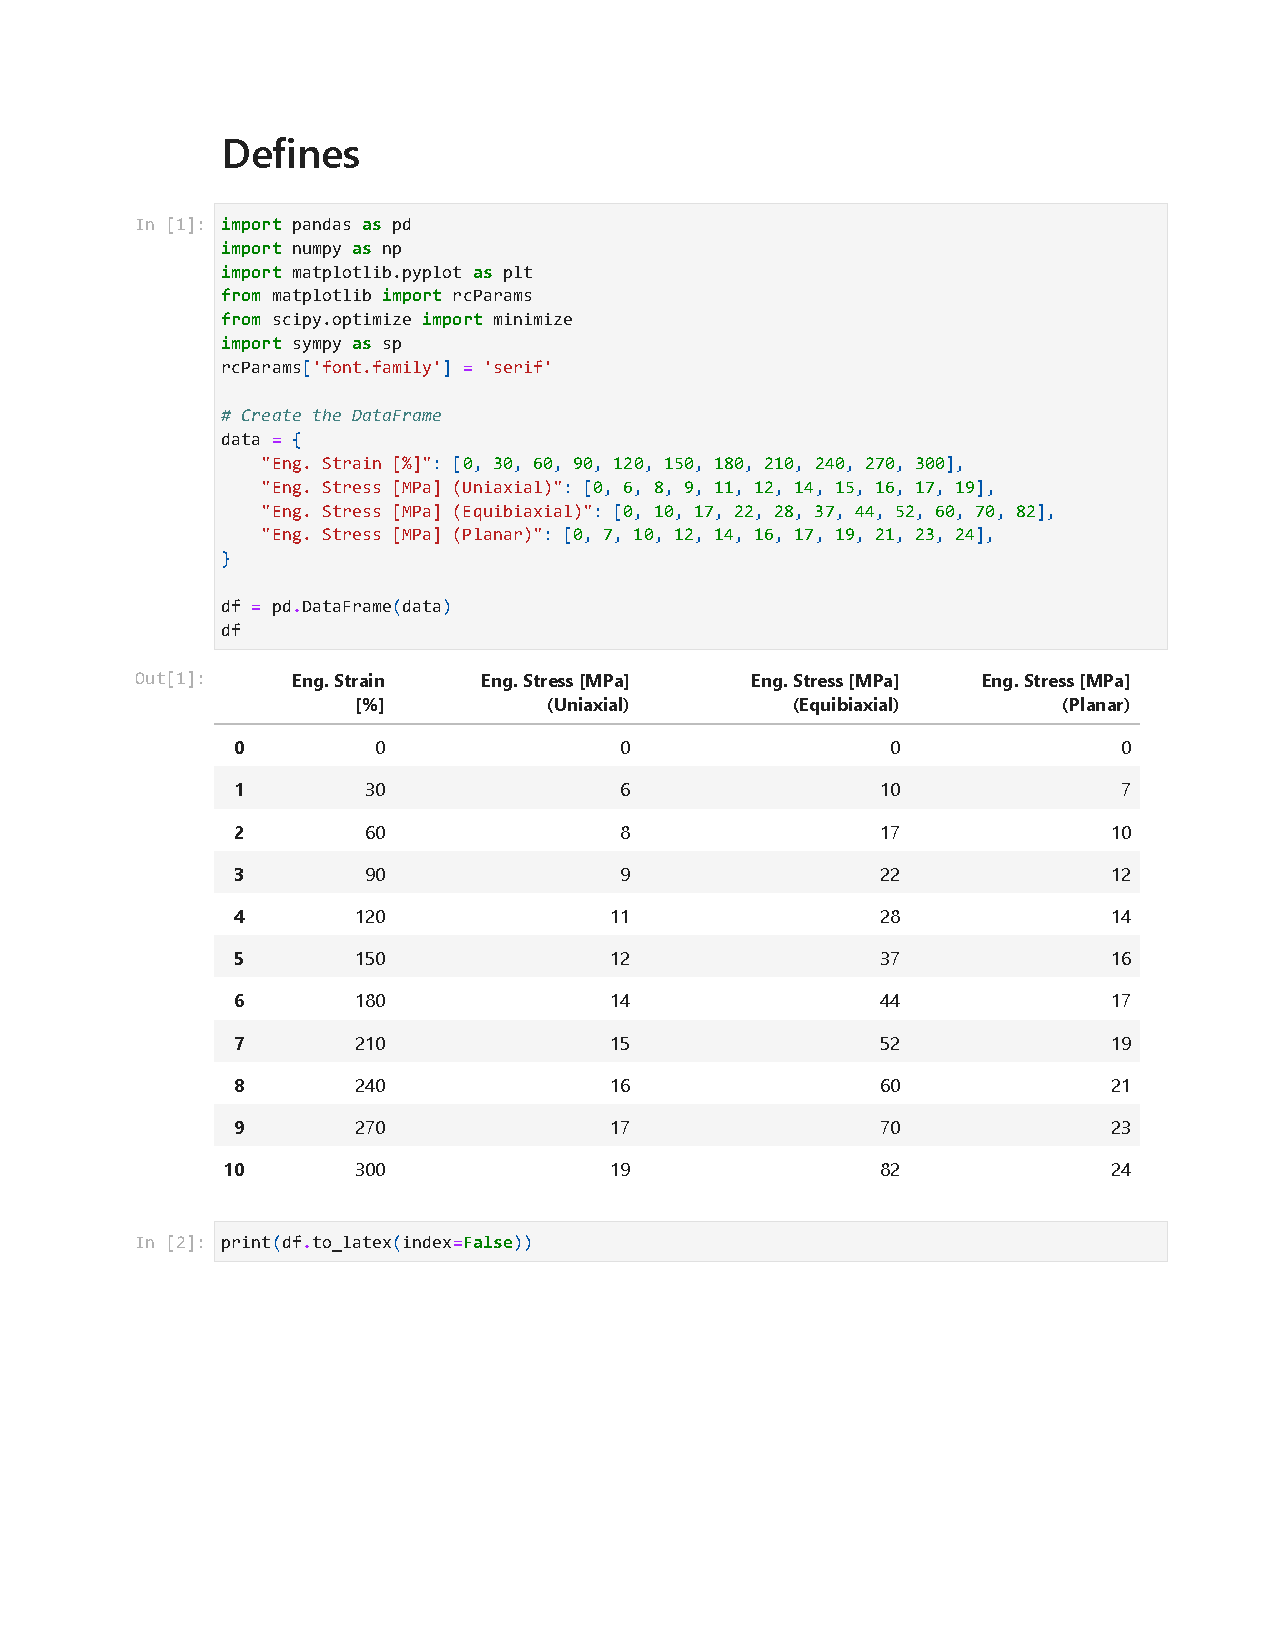
\includepdf[pages=-]{codes.pdf}



\end{document}